\subsection{Task 2.1: Activity diagrams}

    \subsubsection{Request For Printing Service}
    \begin{center}
    \begin{figure}[!htp]
    \begin{center}
     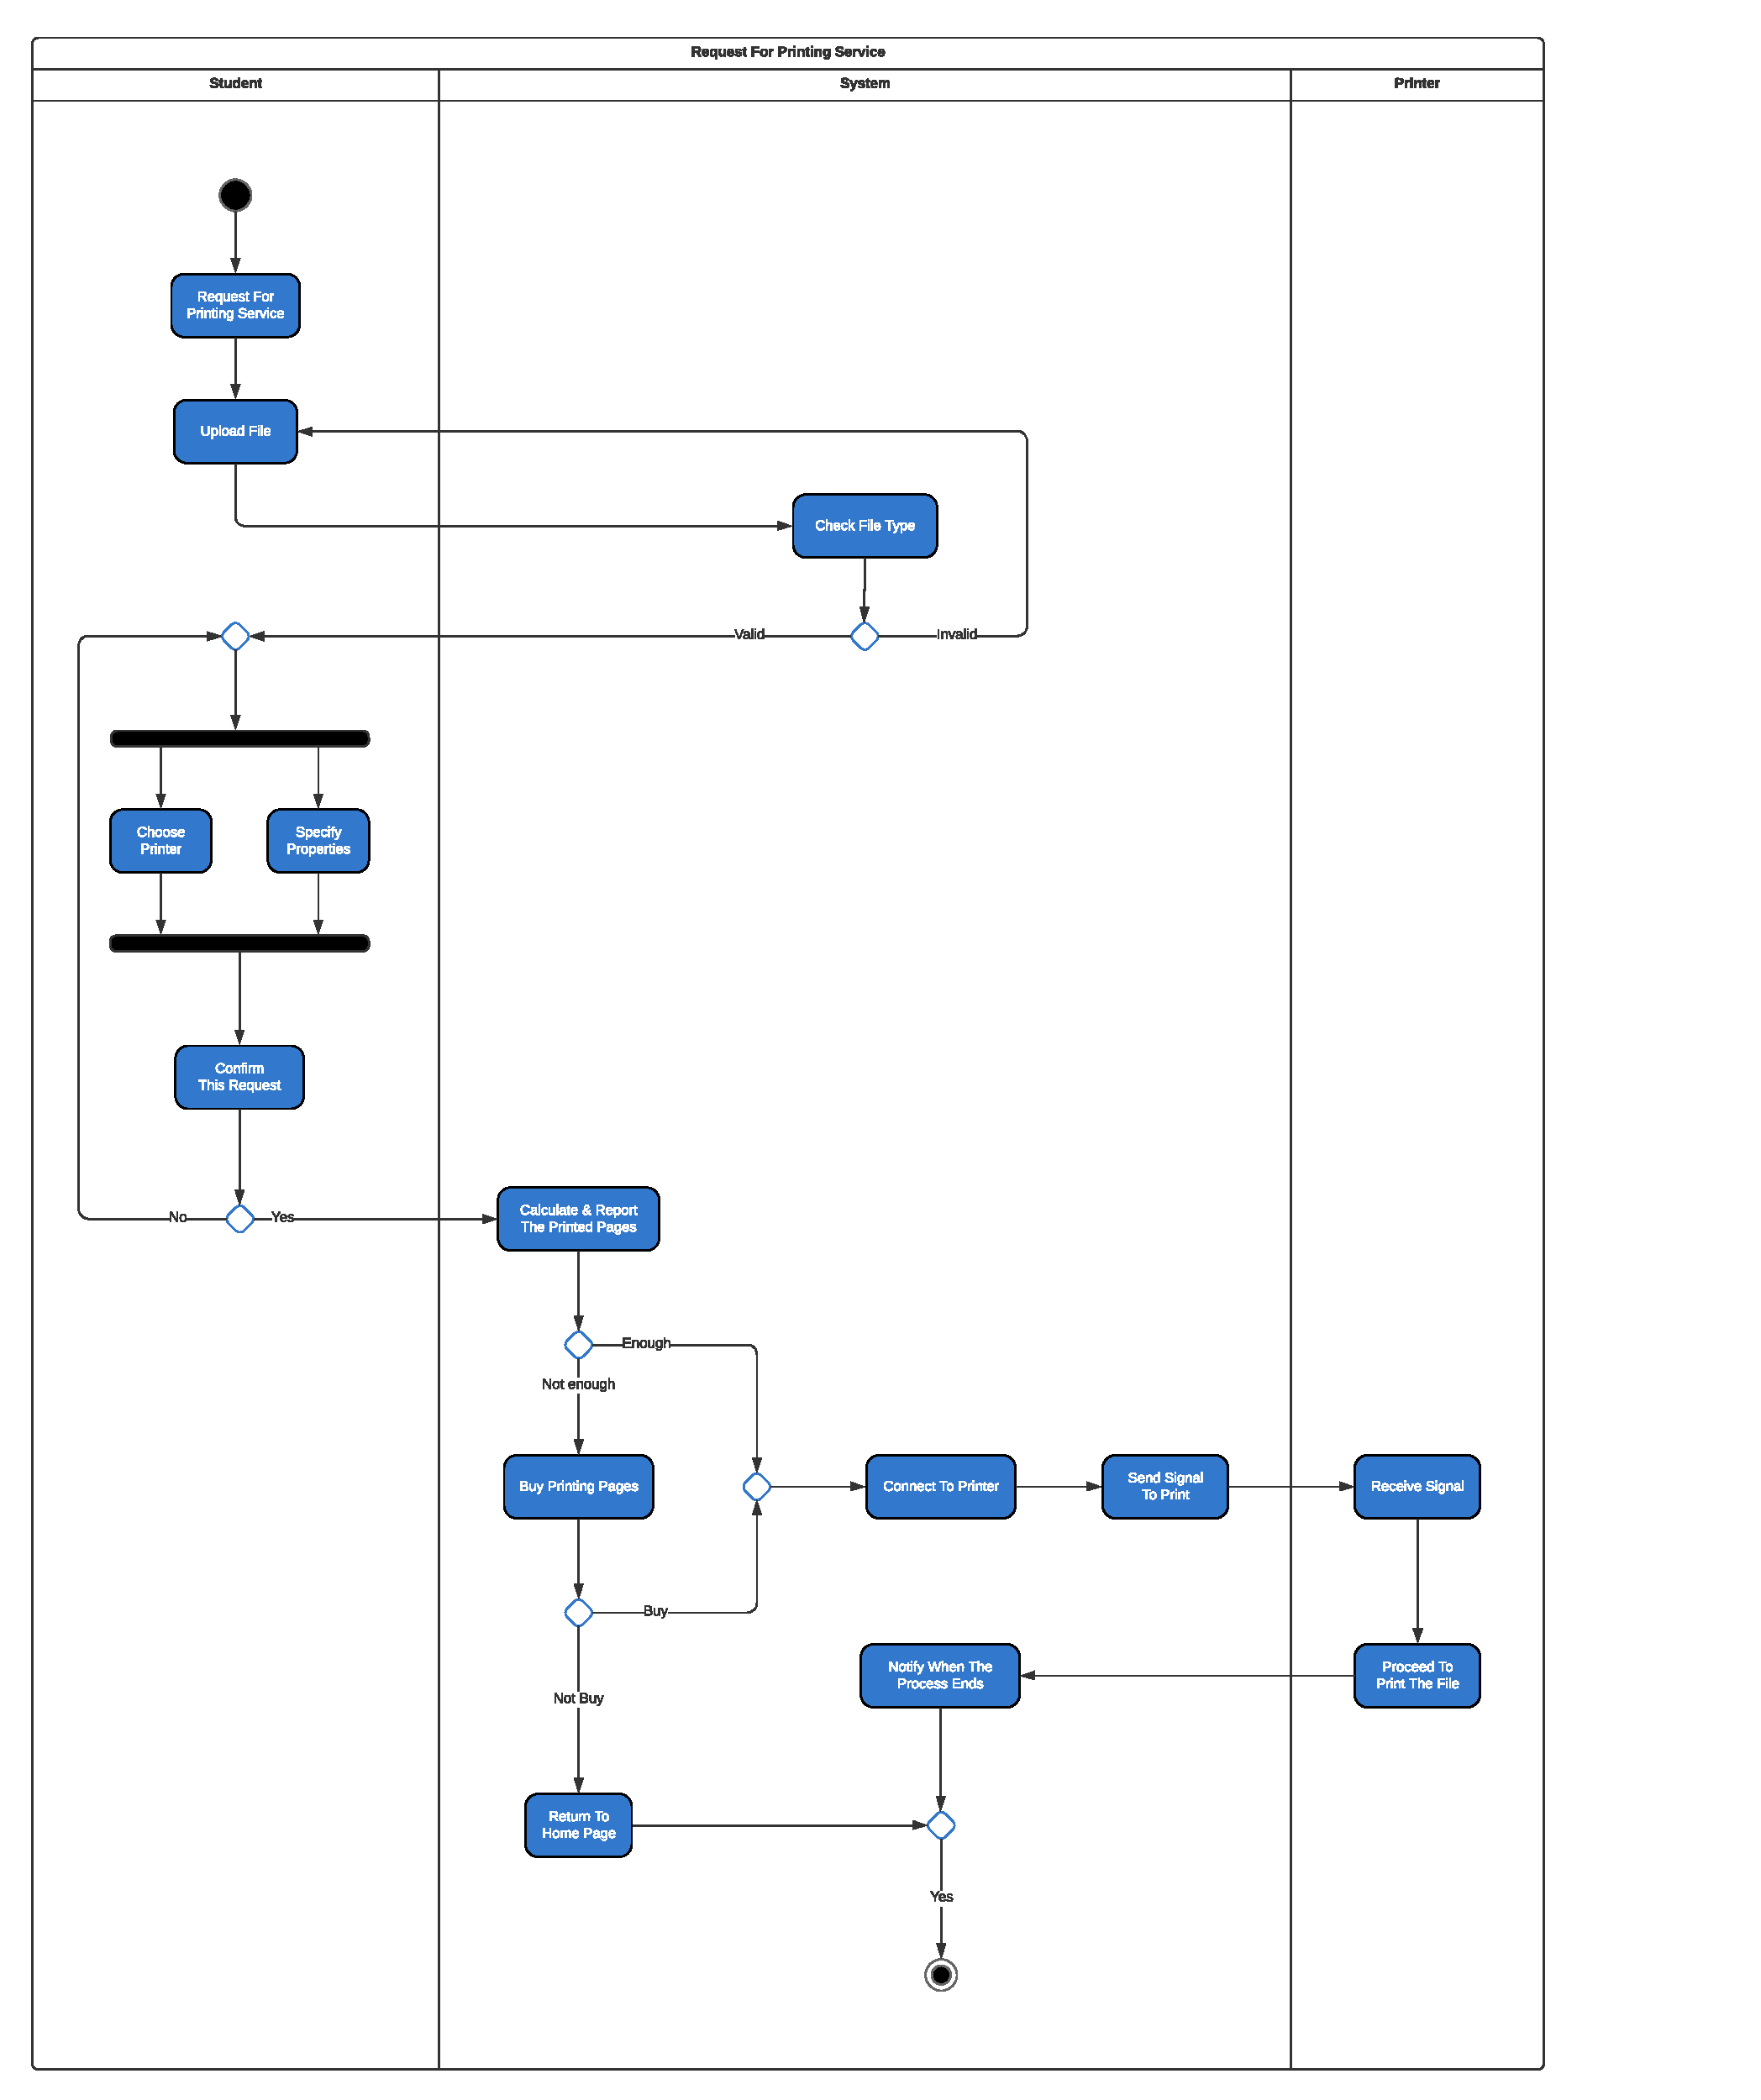
\includegraphics[scale=.4]{images/Task2/ActivityDiagrams/RequestForPrintingService.pdf}
    \end{center}
    \label{refhinh1}
    \end{figure}
    \end{center}
    \newpage
    \textbf{Mô tả:}
    \begin{itemize}
        \item Sinh viên chọn dịch vụ in và tải file cần in lên hệ thống, hệ thống sẽ kiểm tra tính hợp lệ của file:
        \begin{itemize}
            \item Nếu file hợp lệ thì sinh viên sẽ được tiến hành bước tiếp theo.
            \item Nếu file không hợp lệ hệ thống sẽ quay lại bước tải file để sinh viên tải tệp tin khác lên.
        \end{itemize}
        \item Sau khi tải tệp lên sinh viên chọn máy in và cấu hình các thuộc tính in hoặc để mặc định hệ thống.
        \item Sinh viên cần xác nhận để hệ thống tiếp tục bước tiếp theo, bước này nhằm tránh việc sinh viên quên cấu hình các thuộc tính mình cần.
        \item Sau đó hệ thống sẽ tính toán lại số trang mà sinh viên có thể in còn lại và báo cáo lại cho sinh viên:
        \begin{itemize}
            \item Nếu số trang còn lại đủ để phục vụ in tập tin sinh viên vừa tải lên thì hệ thống sẽ tiến hành in cho sinh viên.
            \item Ngược lại, nếu số trang không đủ thì sinh viên được quyền mua thêm hoặc không:
            \begin{itemize}
                \item Nếu sinh viên chọn không mua hệ thống sẽ đưa sinh viên về lại trang chủ.
                \item Nếu sinh viên chọn mua và hoàn tất thanh toán đủ thì hệ thống sẽ tiến hành in tập tin cho sinh viên
            \end{itemize}
        \end{itemize}
        \item Khi đã hoàn thành công việc quản lý máy in, SPSO sẽ đăng xuất hỏi hệ thống.
    \end{itemize}


    \newpage
    \subsubsection{Make Online Payment}
   \begin{center}
    \begin{figure}[!htp]
    \begin{center}
     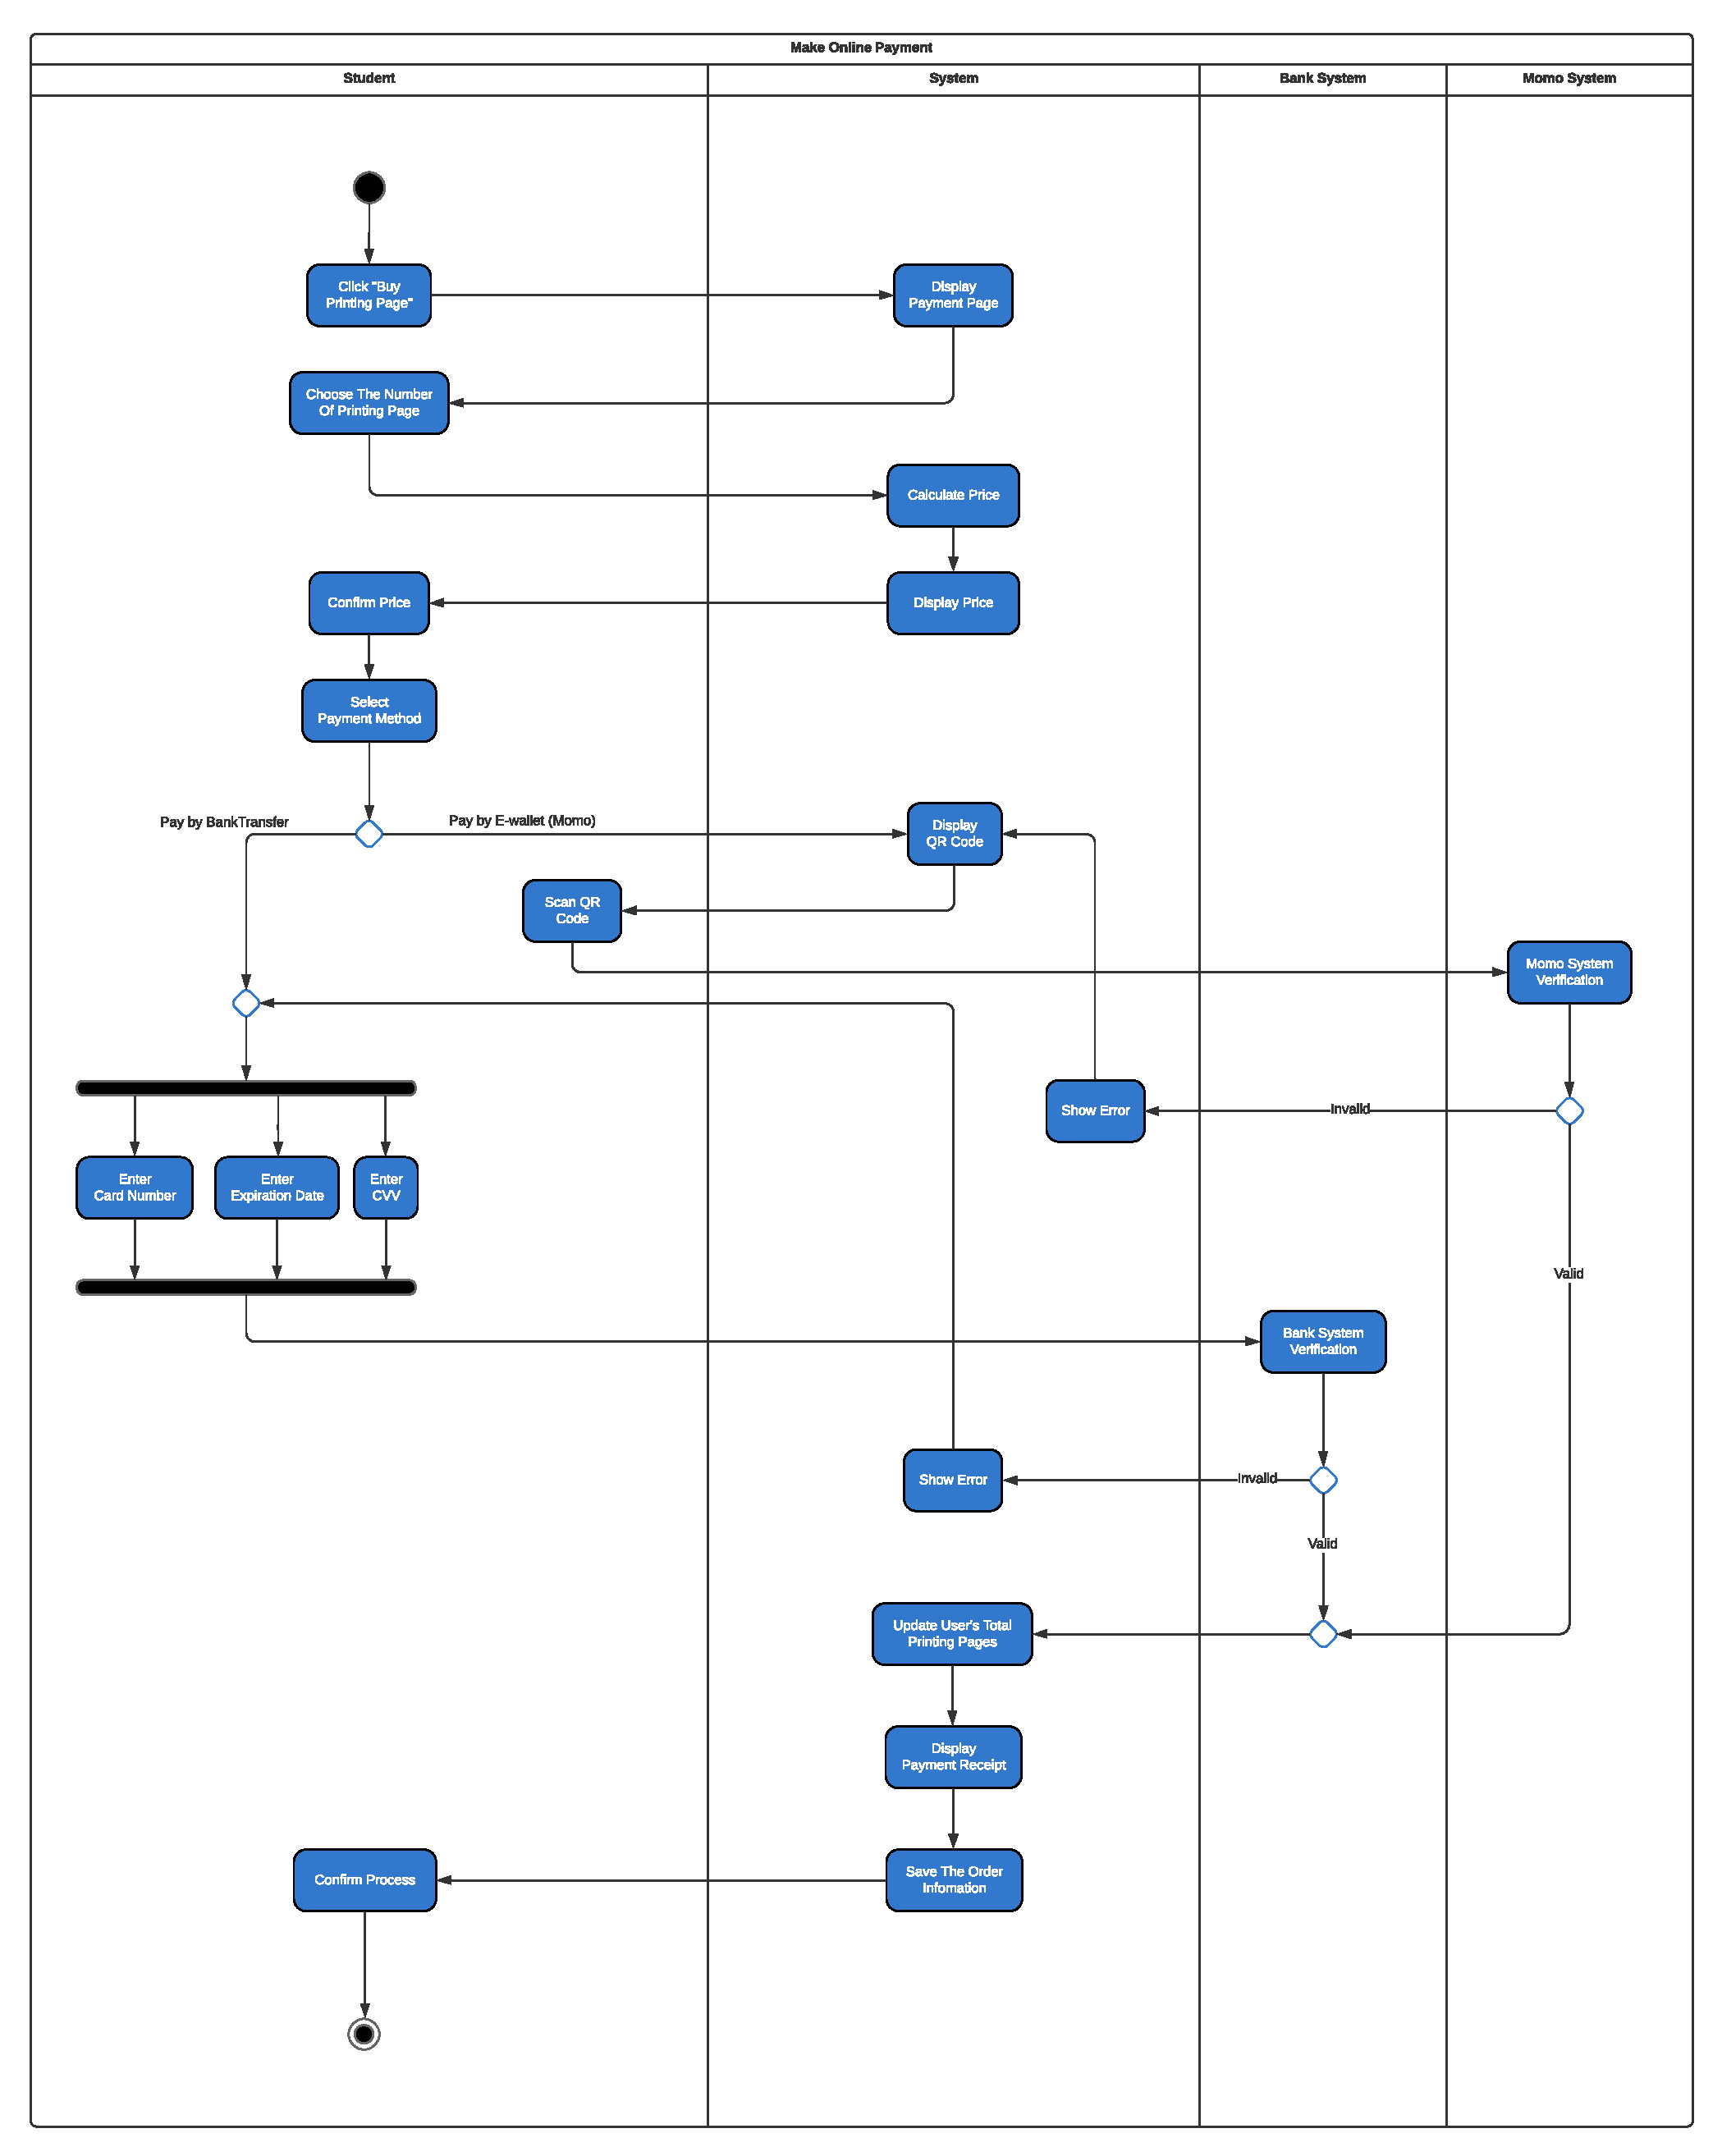
\includegraphics[scale=.4]{images/Task2/ActivityDiagrams/Payment.pdf}
    \end{center}
    \label{refhinh1}
    \end{figure}
    \end{center}
    \newpage
    \textbf{Mô tả:}
    \begin{itemize}
        \item Đầu tiên, khi sinh viên quyết định mua thêm giấy in, họ sẽ lựa chọn dịch vụ mua giấy in trong hệ thống.
        \item Sau khi đăng nhập thành công vào tài khoản của họ, sinh viên có thể tiến hành mua giấy in bằng cách chọn tùy chọn "Mua giấy in." Hệ thống sẽ hiển thị giao diện mua giấy in, nơi sinh viên có thể chỉ định số lượng giấy in mà họ muốn mua.
        \item Hệ thống sẽ dựa vào số lượng giấy in được chọn bởi sinh viên và giá của giấy in tại thời điểm đó để tính toán tổng số tiền cần thanh toán. Sau đó, hiển thị ra màn hình và sinh viên sẽ xem và xác nhận số tiền này.
        \item Sau khi xác nhận giá trị thanh toán, sinh viên có hai lựa chọn thanh toán: sử dụng thẻ Visa hoặc ví điện tử Momo.
        \begin{itemize}
            \item Nếu sinh viên chọn thanh toán bằng thẻ Visa, họ cần cung cấp thông tin thẻ gồm số thẻ, ngày hết hạn và mã bảo vệ. Hệ thống sẽ gửi yêu cầu xác nhận thanh toán đến ngân hàng liên quan.
            \item Nếu sinh viên ưa thích thanh toán qua Momo, hệ thống sẽ hiển thị mã QR. Sinh viên chỉ cần quét mã này, và hệ thống sẽ gửi yêu cầu xác nhận thanh toán đến ví điện tử Momo.
        \end{itemize}
        \item Trong cả hai trường hợp, nếu thanh toán thành công, hệ thống sẽ cập nhật số lượng giấy in trong tài khoản của sinh viên, lưu hóa đơn thanh toán và hiển thị nó để sinh viên có thể xác nhận.
        \item Trong trường hợp thanh toán không thành công, hệ thống sẽ hiển thị thông báo lỗi và đưa quay lại bước thanh toán trước đó để sinh viên có cơ hội sửa lỗi hoặc lựa chọn phương thức thanh toán khác.
    \end{itemize}


    \newpage
    \subsubsection{Manage Printers}
    \begin{center}
    \begin{figure}[!htp]
    \begin{center}
     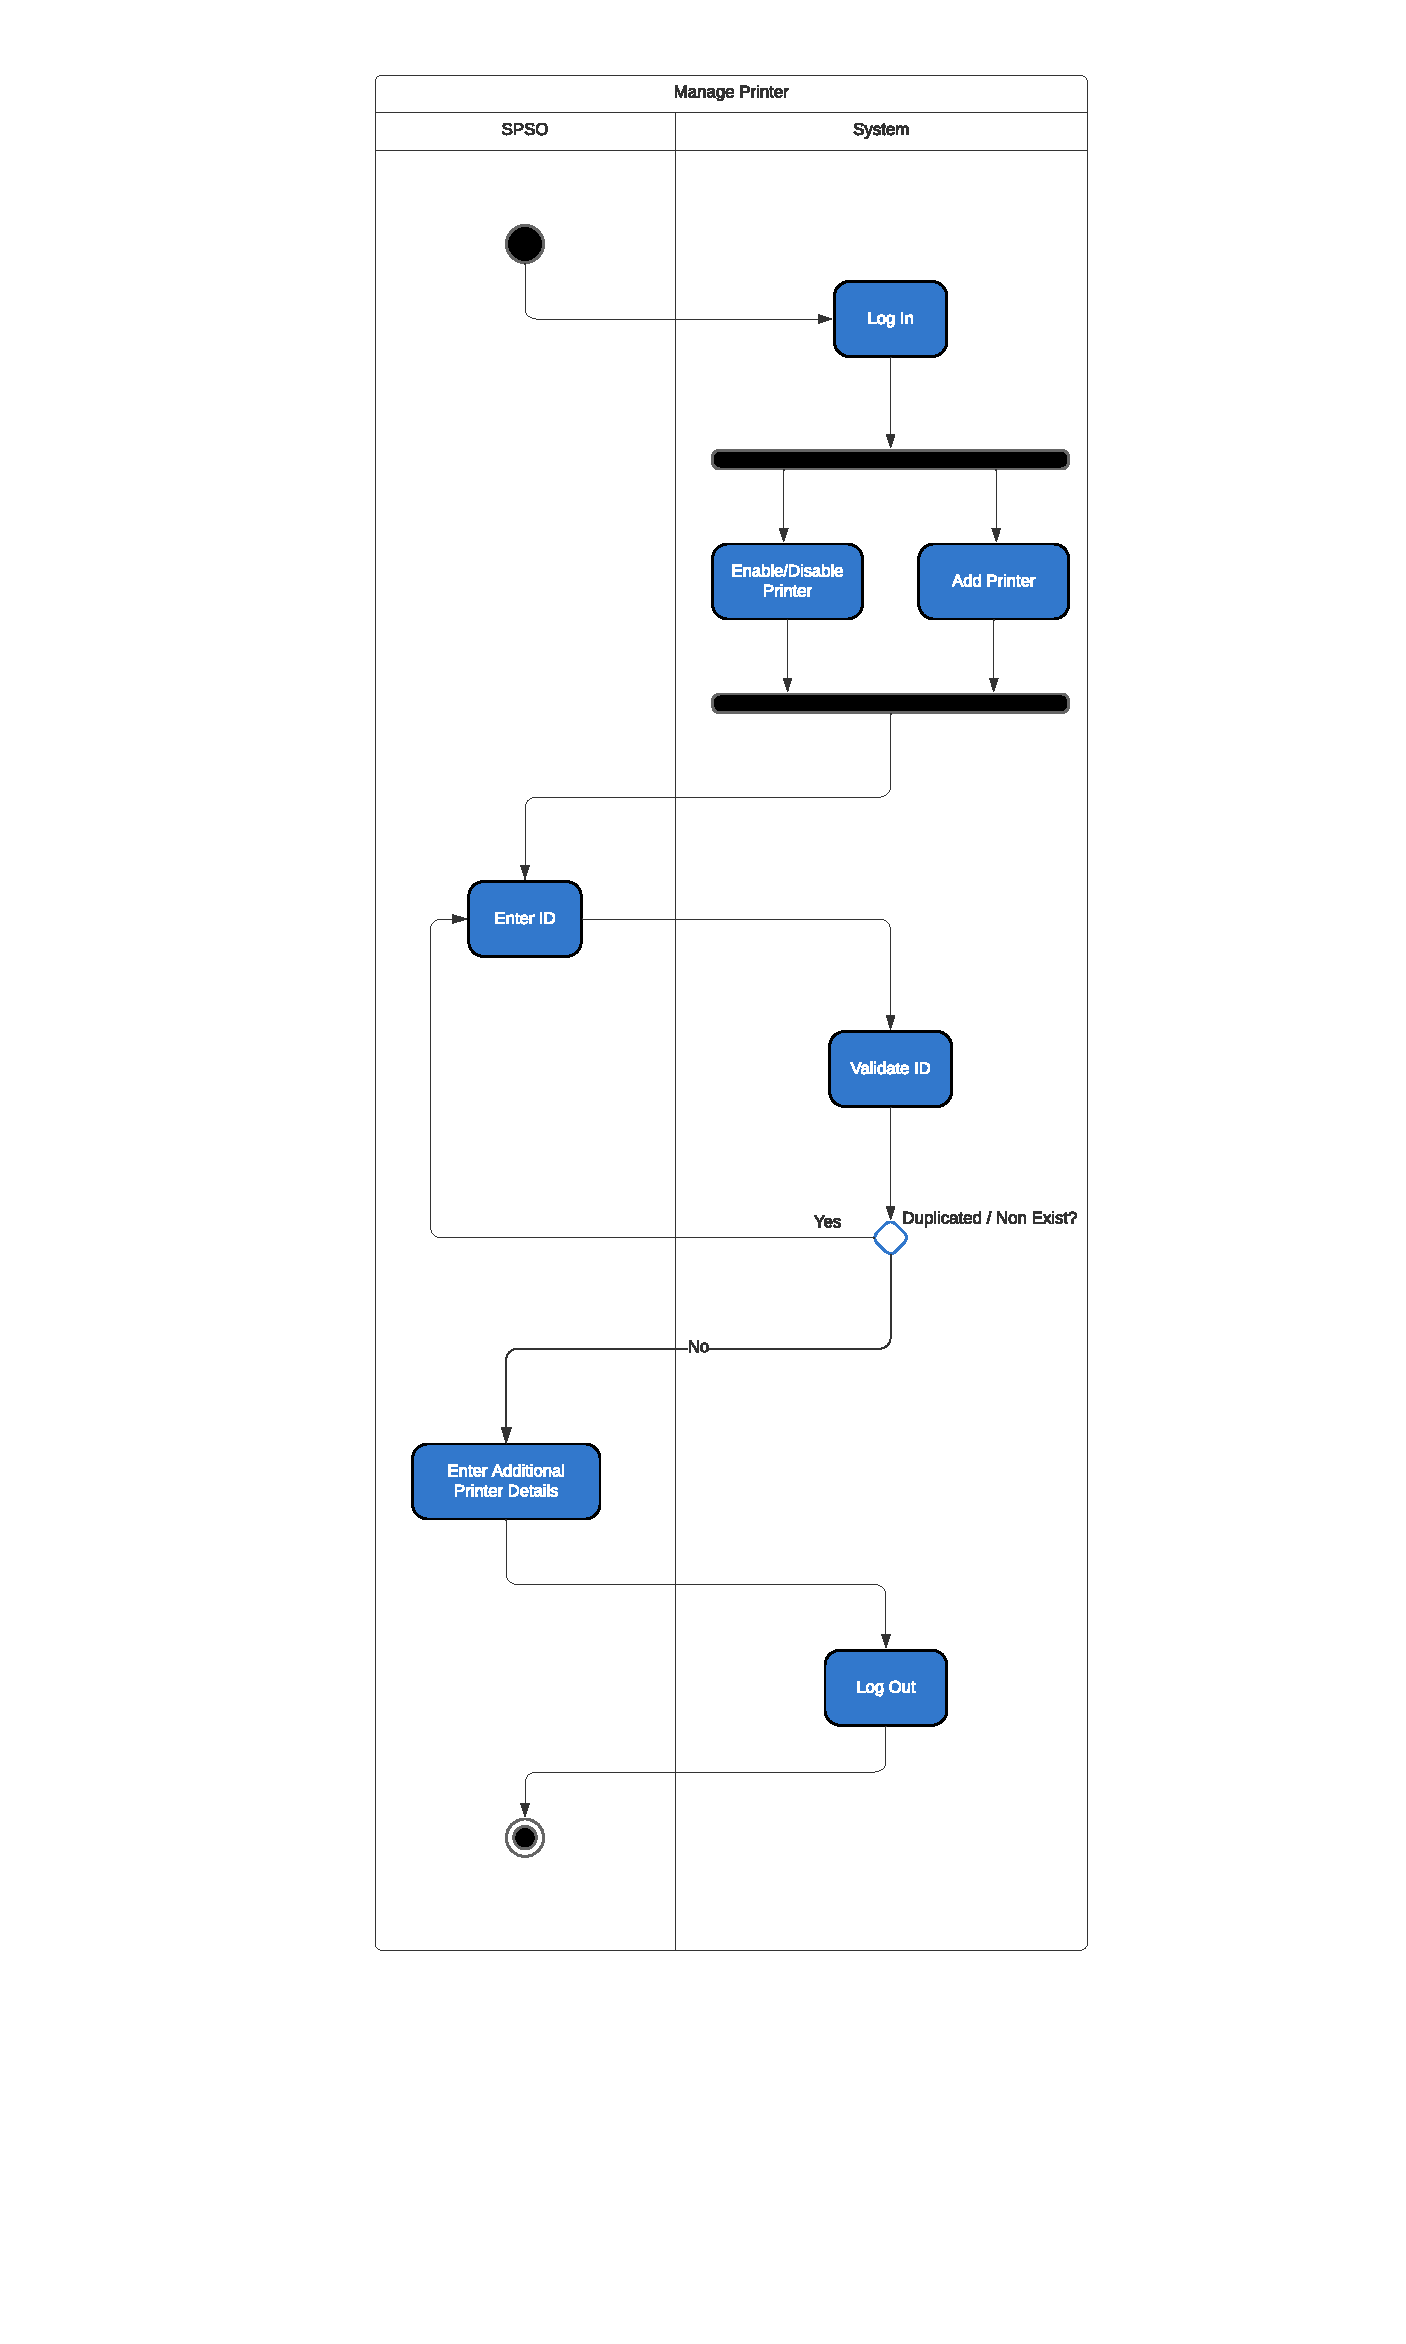
\includegraphics[scale=.45]{images/Task2/ActivityDiagrams/ManagePrinter.pdf}
    \end{center}
    \label{refhinh1}
    \end{figure}
    \end{center}

    \newpage
    \textbf{Mô tả:}
    \begin{itemize}
        \item SPSO sẽ đăng nhập vào hệ thống quản lý máy in qua dịch vụ xác thực HCMUT\_SSO, chọn vai trò (quản lý) và đăng nhập với tài khoản quản lý đã được cấp.
        \item Sau khi đăng nhập thành công, SPSO chọn chức năng quản lý (thêm máy in, bật/tắt máy in):
        \begin{itemize}
            \item Nếu chọn thêm máy in vào hệ thống, SPSO sẽ xác nhận đã có máy in vật lý được lắp đặt tại địa điểm chỉ định hay chưa.
        \end{itemize}
        \item Sau khi xác nhận chức năng, SPSO sẽ phải nhập và xác nhận ID của máy in cần được thêm/bật/tắt đang tồn tại trong hệ thống và hợp lệ, tránh trùng lặp với ID đã có sẵn trong hệ thống.
        \begin{itemize}
            \item Nếu đã chọn chức năng thêm máy in, SPSO sẽ đồng thời điền vào các thông tin của máy in (mẫu mã, địa điểm, ...).
        \end{itemize}
        \item Khi đã hoàn thành công việc quản lý máy in, SPSO sẽ đăng xuất khỏi hệ thống.
    \end{itemize}


    \newpage
    \subsubsection{Configure System}
    \begin{center}
    \begin{figure}[!htp]
    \begin{center}
     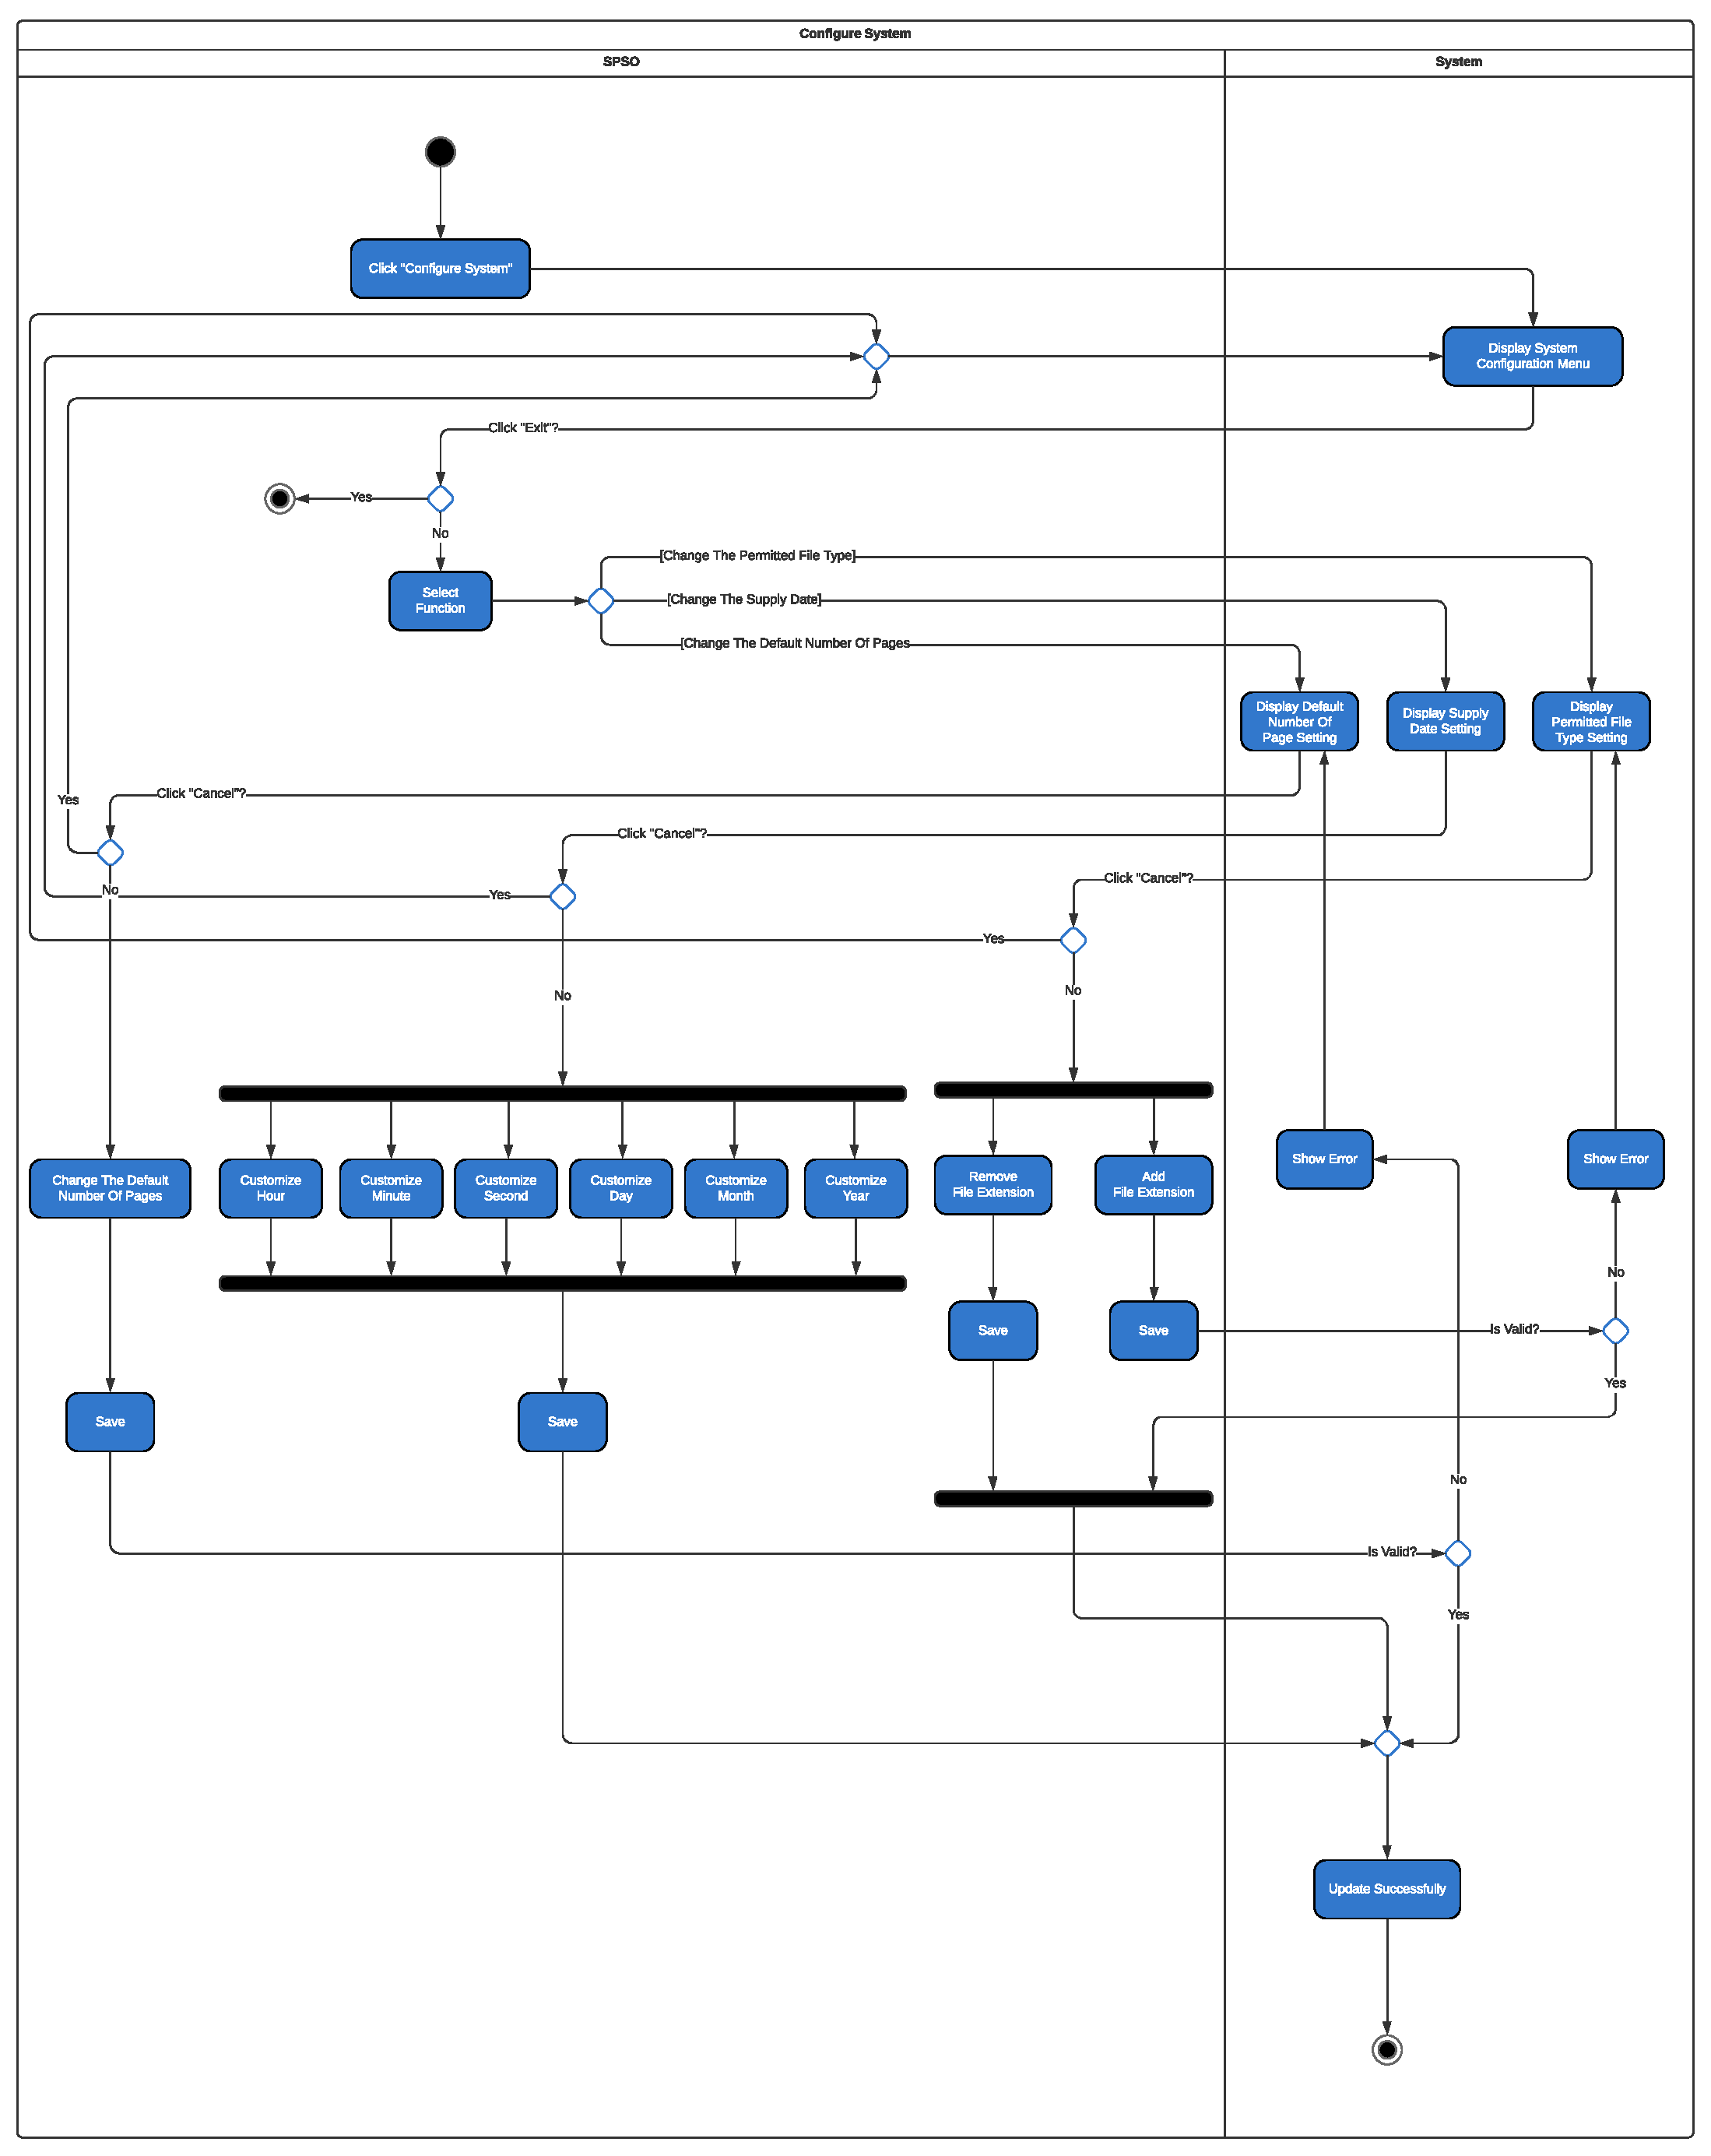
\includegraphics[scale=.4]{images/Task2/ActivityDiagrams/ConfigureSystem.pdf}
    \end{center}
    \label{refhinh1}
    \end{figure}
    \end{center}

    \newpage
    \textbf{Mô tả:}
    \begin{itemize}
        \item SPSO chọn chức năng cấu hình hệ thống trong trang chính, trang tùy chỉnh các cấu hình của hệ thống sẽ hiện ra.\\
        \item SPSO chọn một trong ba chức năng để tiến hành tùy chỉnh.\\
        \begin{itemize}
            \item Nếu SPSO chọn thay đổi số giấy in mặc định, SPSO có thể thay đổi số giấy in mặc định bằng một con số bất kì, con số này phải là số nguyên dương. Khi lưu, hệ thống sẽ kiểm tra sự hợp lệ của số giấy in mặc định mới để xác nhận đã lưu thành công.\\
            \item Nếu SPSO chọn thay đổi thời điểm cung cấp giấy in, SPSO có thể tùy chỉnh các thông số như ngày, tháng, năm, giờ, phút, giây. Các thông số này sẽ được thay đổi bằng các drop down list. Sau đó SPSO cần bấm lưu để thực hiện cập nhật thông số.
            \item Đối với chức năng chỉnh sửa các định dạng tệp tin được cho phép, SPSO có thể thêm định dạng mới hoặc xóa bớt các định dạng đã có sẵn.
        \end{itemize}
    \end{itemize}


    \newpage
    \subsubsection{Log In}
    \begin{center}
    \begin{figure}[!htp]
    \begin{center}
     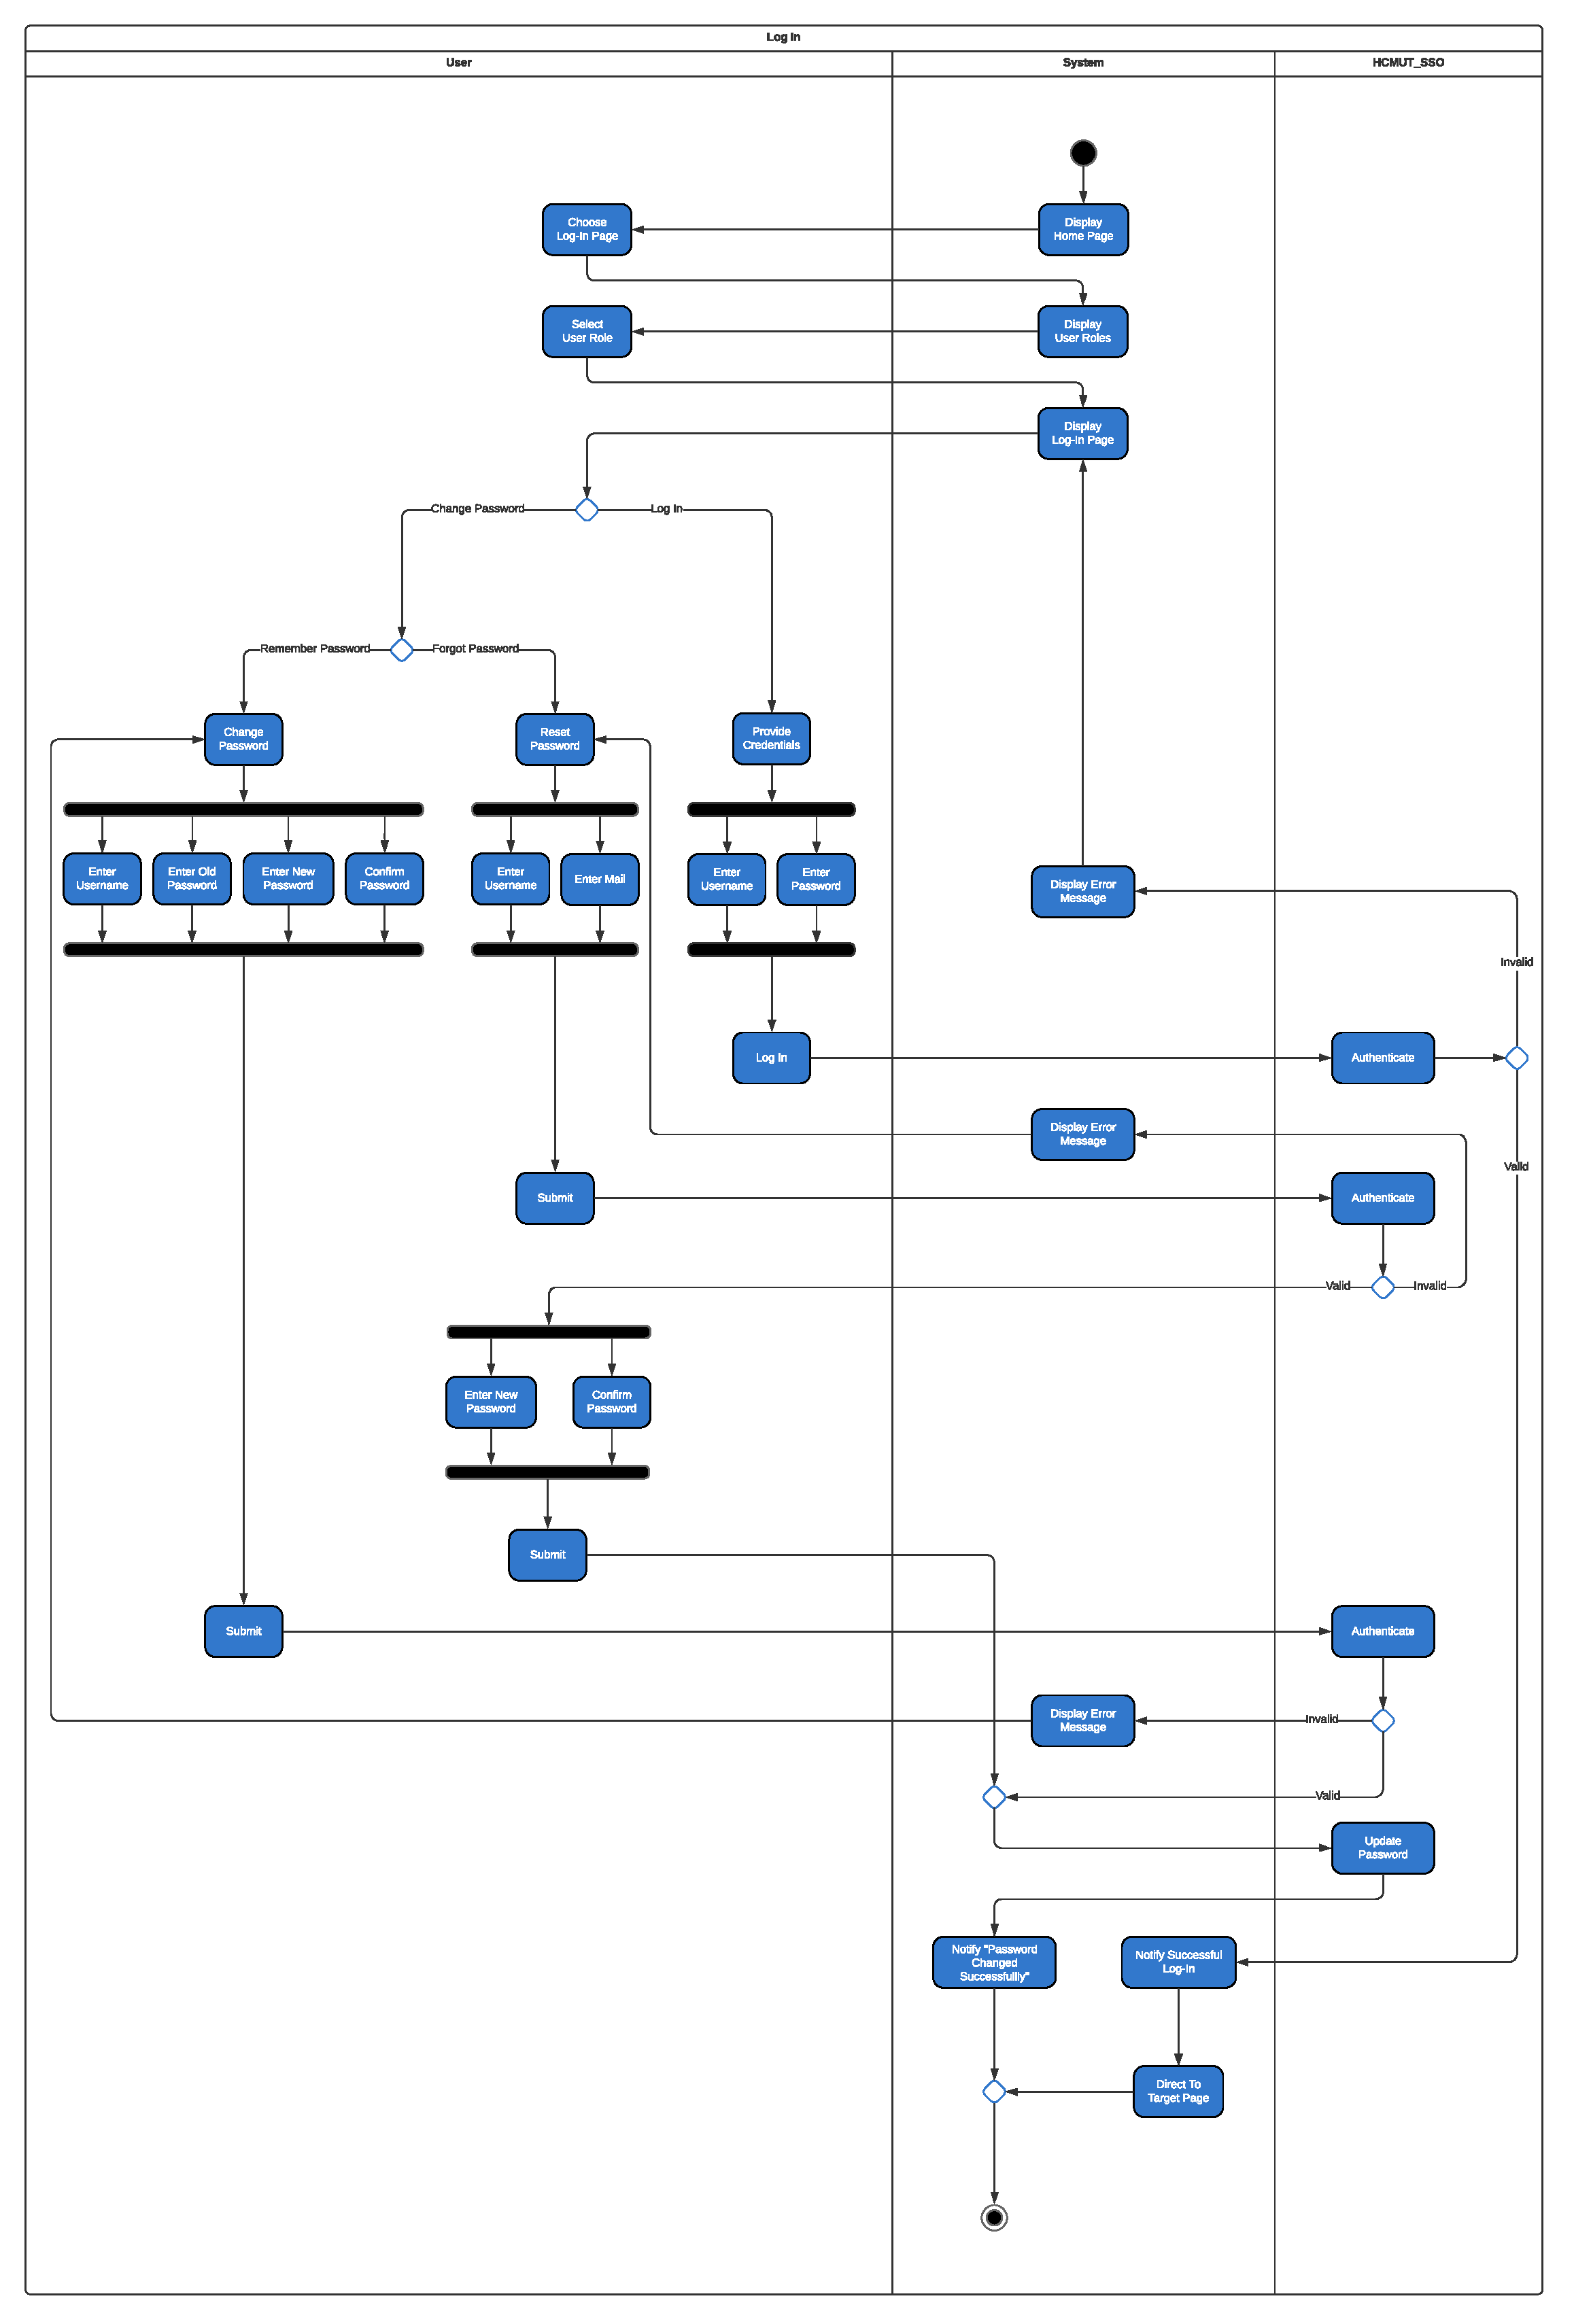
\includegraphics[scale=.34]{images/Task2/ActivityDiagrams/LogIn.pdf}
    \end{center}
    \label{refhinh1}
    \end{figure}
    \end{center}

    \newpage
    \textbf{Mô tả:}
    \begin{itemize}
    \item Người dùng thông qua giao diện để gửi thông tin đăng nhập (username + password) đến hệ thống.
    \item Sau khi nhận được thông tin đăng nhập mà người dùng cung cấp, HCMUT\_SSO sẽ tiến hành xác thực:
        \begin{itemize}
            \item Nếu thông tin đăng nhập được xác nhận thành công (Valid), giao diện sẽ chuyển đến trang sử dụng dịch vụ in (Target Page) để người dùng có thể tiếp tục các lựa chọn trải nghiệm.
            \item Nếu thông tin đăng nhập không xác nhận thành công (Invalid), hệ thống sẽ hiển thị thông báo lỗi và giao diện sẽ chuyển về trang đăng nhập (Log-In Page) để người dùng có thể cung cấp lại thông tin đăng nhập.
        \end{itemize}
    \item Ngoài ra, người dùng có thể thay đổi mật khẩu cho tài khoản của mình:
        \begin{itemize}
            \item Trường hợp người dùng không nhớ mật khẩu hiện tại, người dùng có một sự lựa chọn duy nhất là đổi mật khẩu thông qua mail - Reset Password (username, mail).
            \item Trường hợp người dùng vẫn nhớ mật khẩu hiện tại, người dùng sẽ có thêm một sự lựa chọn khác là đổi mật khẩu thông qua mật khẩu cũ - Change Password (user name , old password).
        \end{itemize}
    \end{itemize}